\documentclass{amsart}
\usepackage{amsmath}
\usepackage{amssymb}
\usepackage{bbm}
\usepackage{a4wide}
\usepackage{sagetex}
\usepackage{tikz}

\parindent=0pt
\parskip\smallskipamount

\let\set\mathbbm
\def\<#1>{\langle#1\rangle}
\let\ideal\unlhd
\def\i{\mathrm{i}}
\def\e{\mathrm{e}}

\def\Bold#1{\mathbf{#1}}

\newtheorem{thm}{Theorem}
\newtheorem{prop}{Proposition}
\newtheorem{defn}{Definition}
\newtheorem{conj}{Conjecture}

\newcommand\todo[1][.]{\edef\tmpa{.}\edef\tmpb{#1}%
  \ifx\tmpa\tmpb
    \typeout{To Be on page \thepage}\fbox{\bf To Be}
  \else
    \typeout{To Be on page \thepage: #1}\fbox{{\bf To Be:} #1}
  \fi
}

\begin{document}

 \author[Manuel Kauers, Maximilian Jaroschek, Fredrik Johansson]
   {Manuel Kauers\,$^\ast$, Maximilian Jaroschek\,$^\ast$, Fredrik Johansson\,$^\ast$}
 \address{Manuel Kauers, Research Institute for Symbolic Computation (RISC), J. Kepler University Linz, Austria}
 \email{mkauers@risc.uni-linz.ac.at}
 \address{Maximilian Jaroschek, Research Institute for Symbolic Computation (RISC), J. Kepler University Linz, Austria}
 \email{mjarosch@risc.uni-linz.ac.at}
 \address{Fredrik Johansson, Research Institute for Symbolic Computation (RISC), J. Kepler University Linz, Austria}
 \email{fjohanss@risc.uni-linz.ac.at}
 \thanks{$^\ast$ Supported by the Austrian FWF grant Y464-N18.}

 \title{Ore Polynomials in Sage}

 \begin{abstract}
We present a Sage implementation of Ore algebras. The main features for the most
common instances include basic arithmetic and actions; gcrd and lclm; D-finite
closure properties; natural transformations between related algebras; guessing;
desingularization; solvers for polynomials, rational functions and (generalized)
power series. This paper is a tutorial on how to use the package.
 \end{abstract}

 \maketitle

%%% page limit: 20, goal: 15--20.

\section{Introduction}

In computer algebra, objects are often described implicitly through equations
they satisfy. For example, the exponential function $\exp(x)$ is uniquely
specified by the linear differential equation $f'(x)-f(x)=0$ and the initial
value $f(0)=1$.  Likewise, the sequence $F_n$ of Fibonacci numbers is uniquely
determined by the linear recurrence $F_{n+2}-F_{n+1}-F_n=0$ and the two initial
values $F_0=0$,~$F_1=1$.  Especially for representing functions or sequences
that cannot be expressed in ``closed form'', the differential or difference
equations they may satisfy provide an attractive way to store them on the
computer. The question is then how to calculate with objects which are given in
this form.

Algorithms for Ore algebras provide a systematic answer to this
question~\cite{..,..}.  Invented in the early 20th century~\cite{..} with the
objective of providing a unified theory for various kinds of linear operators,
they have been used for many years in computer algebra systems, for example in
the Maple packages gfun~\cite{..} and mgfun~\cite{..}, in the Mathematica
packages by Mallinger~\cite{..} and Koutschan~\cite{..,..}, and
elsewhere~\cite{..}. 

The purpose of this paper is to introduce an implementation of a collection of
algorithms related to Ore algebras for the computer algebra system
Sage~\cite{..}. It is addressed to first-time users who are already familiar
with Sage, and with the theory of Ore algebras and its use for doing symbolic
computation related to special functions. Readers unfamiliar with Sage are referred
to~\cite{..}, and readers unfamiliar with Ore algebras may wish to consult the
recent tutorial~\cite{..} and the references given there for an introduction to
the subject.

At the time of writing, the package we describe here is still under construction
and has not yet been incorporated into the official Sage distribution. Readers
who want to try it out are invited to download the current latest version from 
[URL] and are encouraged to send us bug reports and other comments. We hope 
that the community will find the code useful.

Creating an Ore algebra object is easy. The following instructions show how to 
load the code and then create an Ore algebra $A$ of linear differential operators
and an Ore algebra $B$ of recurrence operators. Observe the correct application
of the respective commutation rules in both cases. 

\begin{sageexample}
  sage: load("ore_algebra.py", "guessing.py");  #### TO BE FIXED ####
  sage: R.<x> = PolynomialRing(ZZ); A.<Dx> = OreAlgebra(R)
  sage: A
  sage: A.random_element()
  sage: Dx*x
  sage: B.<Sx> = OreAlgebra(R)
  sage: B
  sage: Sx*x
\end{sageexample}

More details on the construction of Ore algebras are given in the following section.
Also Ore algebras with several generators are already supported. However, so far we offer
no functionality beyond addition and multiplication for these. More functionality 
is available for algebras with one generator. We describe some of it in 
Section~\ref{sec:3}. Even more functionality has been implemented for special 
algebras like the ones created above, which are most frequently used in practice. 
See Section~\ref{sec:4} for an overview. Finally, the package also comes with a 
fine tuned guessing engine, whose main features we describe in Section~\ref{sec:5}.

\section{Ore Algebras}

An Ore algebra is determined by a base ring and a finite number of generators.
In the examples above, the base ring was $\Bold{Z}[x]$, and the generators were
$\mathrm{Dx}$ and $\mathrm{Sx}$, respectively. If no other information is provided
in the arguments, the \verb|OreAlgebra| constructor chooses the nature of the 
generators according to their name: a generator called $\mathrm{Dt}$ represents
the standard derivation $d/dt$ acting on the generator $t$ of the base ring, 
a generator called $Sn$ represents the standard shift operator sending the
generator $n$ of the base ring to $n+1$. 

For this way of generating algebras, generator names must be composed of
one of the following single-letter prefixes followed by the name of a generator
of the base ring. 

\begin{center}
  \begin{tabular}{|c|c|c|}\hline
    Prefix & Name & Commutation rule \\\hline
     D & Standard derivation $d/dx$ & $\mathrm{Dx}\,x=x\,\mathrm{Dx}+1$ \\
     S & Standard shift $x\leadsto x+1$ & $\mathrm{Sx}\,x=(x+1)\,\mathrm{Sx}$ \\
     T or $\Theta$ & Eulerian derivation $x\,d/dx$ & $\mathrm{Tx}\,x=x\,\mathrm{Tx}+x$ \\
     F or $\Delta$ & Forward difference $\Delta_x$ & $\mathrm{Fx}\,x=(x+1)\mathrm{Fx}+1$ \\
     Q & $q$-shift $x\leadsto q\,x$ & $\mathrm{Qx}\,x=q\,x\,\mathrm{Qx}$ \\
     J & $q$-derivation (``Jackson derivation'') & $\mathrm{Jx}\,x=q\,x\,\mathrm{Jx}+1$ \\ 
     C & commutative generator & $\mathrm{Cx}\,x = x\,\mathrm{Cx}$ \\\hline
  \end{tabular}
\end{center}

For the $q$-shift and the $q$-derivation, the base ring must contain an element~$q$.
The element playing the role of $q$ can be specified as an optional argument. 

\begin{sageexample}
  sage: R.<x> = PolynomialRing(ZZ['q'])
  sage: A.<Qx> = OreAlgebra(R)
  sage: Qx*x
  sage: A.<Qx> = OreAlgebra(R, q=2)
  sage: Qx*x
\end{sageexample}

In general, the commutation rules of a generator~$X$ of an Ore algebra~$A$ with
base ring~$R$ are governed by two maps, $\sigma\colon R\to R$ and $\delta\colon R\to R$,
where $\sigma$ is a ring endomorphism (i.e., $\sigma(a+b)=\sigma(a)+\sigma(b)$ and
$\sigma(ab)=\sigma(a)\sigma(b)$ for all $a,b\in R$) and $\delta$ is a skew-derivation
for $\sigma$ (i.e., $\delta(a+b)=\delta(a)+\delta(b)$ and $\delta(ab)=\delta(a)b
+\sigma(a)\delta(b)$ for all $a,b\in R$). With two such maps being given, the
generator $X$ satisfies the commutation rule $Xa=\sigma(a)X+\delta(a)$ for every
$a\in R$. If there is more than one generator, then each of them has its own pair
of maps $\sigma,\delta$. Different generators commute with each other; 
noncommutativity only takes place ``between'' generators and base ring elements. 

It is possible to create an Ore algebra with user specified commutation rules.
In this form, each generator must be declared by a tuple $(X,\sigma,\delta)$, 
where $X$ is the name of the generator (a string), and $\sigma$ and $\delta$
are dictionaries which contain the images of the generators of the base
ring under the respective map. Here is how to specify an algebra of difference
operators in this way:

\begin{sageexample}
  sage: R.<x> = ZZ['x']
  sage: A = OreAlgebra(R, ('X', {x:x+1}, {x:1}))
  sage: X = A.gen()
  sage: X*x
\end{sageexample}

As another example, here is how to define an algebra of differential operators 
whose base ring is a differential field $K=\set Q(x,y,z)$ where $y$ represents
$\exp(x)$ and $z$ represents $\log(x)$:

\begin{sageexample}
  sage: K = ZZ['x','y','z'].fraction_field()
  sage: x,y,z = K.gens()
  sage: A = OreAlgebra(K, ('D', {}, {x:1, y:y, z:1/x}))
  sage: D = A.gen()
  sage: D*x, D*y, D*z
\end{sageexample}

In the dictionary specifying~$\sigma$, omitted generators are understood to be
mapped to themselves, so that \verb|{}| in the definition of $A$ in the example
above is equivalent to \verb|{x:x,y:y,z:z}|.  Likewise, in the dictionaries
specifying~$\delta$, omitted generators are understood to be mapped to zero.

For Ore algebras with several generators, it is possible to mix specifications
of generators via triples $(X,\sigma,\delta)$ with generators using the naming
convention shortcuts as explained before. Continuing the previous example,
here is a way to define an algebra $A$ over $K$ with two generators, a $D$ 
that behaves like before, and in addition an $Sx$ which acts like the standard
shift on~$x$.

\begin{sageexample}
  sage: A = OreAlgebra(K, ('D', {}, {x:1, y:y, z:1/x}), 'Sx')
  sage: D, Sx = A.gens()
  sage: D*x, Sx*x
\end{sageexample}

Not every ring is suitable as base ring of an Ore algebra. Base rings must
themselves be polynomial rings (univariate or multivariate), or fraction 
fields of polynomial rings. Their base rings in turn may be either $\set Z$,
$\set Q$, a prime field $GF(p)$, or a number field $\set Q(\alpha)$, or
--- recursively --- some ring which itself would be suitable as base ring
of an Ore algebra. 

\begin{sageexample}
  sage: ZZ['x'].fraction_field()['y','z'] ### OK
  sage: GF(1091)['x','y','z']['u'] ### OK
  sage: ( ZZ['x','y','z'].quotient_ring(x^2+y^2+z^2-1) )['u'] ### not OK
  sage: GF(9, 'a')['x'] ### not OK
\end{sageexample}

Note that the maps $\sigma$ and $\delta$ must leave all the elements of
the base ring's base ring fixed. They may only have nontrivial images for
the top level generators. 

The constituents of an Ore algebra $A$ can be accessed through the methods
summarized in the following table. Further methods can be found in the 
documentation. 

\begin{center}
  \begin{tabular}{|l|p{.55\hsize}|}
    \hline
    Method name & short description \\\hline
    \verb|associated_commutative_algebra()| & returns a polynomial ring with the
       same base ring as $A$ and whose generators are named like the generators
       of~$A$\\
    \verb|base_ring()| & returns the base ring of $A$\\
    \verb|delta(i)| & returns a callable object representing the delta map
       associated to the $i$th generator (default: $i=0$) \\
    \verb|gen(i)| & returns the $i$th generator (default: $i=0$)\\
    \verb|sigma(i)| & returns a callable object representing the sigma map
       associated to the $i$th generator (default: $i=0$) \\
    \verb|var(i)| & returns the name of the $i$th generator (default: $i=0$)\\\hline
  \end{tabular}
\end{center}

\smallskip

Examples: 

\begin{sageexample}
  sage: R.<x> = ZZ['x']; A.<Dx> = OreAlgebra(R)
  sage: A
  sage: A.associated_commutative_algebra()
  sage: A.base_ring()
  sage: A.gen()
  sage: s = A.sigma(); d = A.delta(); 
  sage: s(x^5), d(x^5)
\end{sageexample}

\section{Ore Polynomials}\label{sec:3}

arithmetic, lclm, gcrd, action, coercion and conversion, pretty printing, 
coefficient extraction, closure properties, associate solutions. 

\section{Special Methods for Standard Algebras}\label{sec:4}

special methods available for univ algebras with univ algebra as ground ring

\subsection{Differential Operators}

D and theta

\subsection{Recurrence Operators}

We compute an annihilator for the sequence
$c(n) = \sum_{k=0}^n 1 / k!$:

\begin{sageexample}
  sage: R.<n> = ZZ[]; RS.<Sn> = OreAlgebra(R, 'Sn')
  sage: inverse_factorials = (n + 1) * Sn - 1
  sage: partial_sums = inverse_factorials.annihilator_of_sum()
  sage: partial_sums
\end{sageexample}

The \verb|to_list| method returns the first few values of a sequence,
given the initial values:

\begin{sageexample}
  sage: L = partial_sums.to_list([1, 2], 8)
  sage: L
  sage: N(L[7])
\end{sageexample}

In some cases (for example when the base ring is $\mathbb{Z}$ or
$\mathbb{Z}[x]$), isolated values can be
computed asymptotically faster for large $n$ using the binary splitting
technique.
The \verb|forward_matrix_bsplit| method, called with argument $n$,
returns a matrix $P$ and a denominator $Q$ such that $P / Q$ multiplied a
column vector of initial values $c_0, c_1, \ldots$
yields $c_n, c_{n+1}, \ldots$.
This way, computing $10^5$ digits of $e$ takes a fraction of a second:

\begin{sageexample}
  sage: e_approx = N(e, 400000)
  sage: P, Q = partial_sums.forward_matrix_bsplit(25600)
  sage: u = Matrix([[e_approx], [e_approx]]) - P * Matrix([[1], [2]]) / Q
  sage: u.change_ring(RealField(20))
\end{sageexample}




\subsection{The $q$-Case}

J and Q

\section{Guessing}\label{sec:5}

[[CITE RUBEY.]]

Guessing is one of the most popular features of software packages like gfun.  It
is a technique for detecting patterns in sequences of numbers, which is often
used in combinatorics. The basic idea is simple. If we are given a finite array
of numbers, though of as the first terms of an infinite sequence, we may want to
know whether this sequence satisfies a recurrence. The algorithm behind a
guessing engine searches for small equations matching the given data.
Generically, no such equations exist, so if some are found, it is fair to
``guess'' that they are in fact valid equations for the whole infinite sequence.

We provide a guessing function which takes as input a list of terms and an Ore
algebra, and returns as output an operator which matches the given data and
which, in some measure, would be unlikely to exist for random data.

\begin{sageexample}
  sage: data = [ 0, 1, 1, 2, 3, 5, 8, 13, 21, 34, 55 ]
  sage: L = guess(data, OreAlgebra(ZZ['n'], 'Sn'))
  sage: L
  sage: L(data)
  sage: M = guess(data, OreAlgebra(ZZ['x'], 'Dx'))
  sage: M
  sage: M(x/(1-x-x^2))
\end{sageexample}

If an algebra of differential operators is supplied as second argument, the data
is understood as the first few coefficients of a power series. The output
operator is expected to have this power series as solution.

It can happen that the procedure is unable to find an operator matching the 
given data. In this case, an exception is raised. There are two possible 
explanations for such an event. Either the sequence in question does not 
satisfy any equations, or it does but the equations are so big that more
data is needed to detect them. 

A number of options are available for governing the search for relations.  In
order to explain them, we first need to give some details on the underlying
algorithms. For simplicity of language, we restrict here to the case of
recurrence operators. The situation for differential operators is very similar.

For the most typical situations, there are two important hyperbolas. One
describes the region in the $(r,d)$-plane consisting of all points for which
there exists an operator of order~$r$ and degree~$d$ truly satisfied by the
sequence in question. (See~\cite{..} for an explanation why the boundary of this
region is usually a hyperbola.) The second describes the region of all points
$(r,d)$ for which an operator of order~$r$ and degree~$d$ can be detected when
$N$ terms are provided as input. This region is determined by the requirement
$(r+1)(d+2)<N$. 

The method tests a sequence of points $(r_1,d_1)$, $(r_2,d_2)$, \dots\ right
below this second parabola. Success at a point $(r_i,d_i)$ means that some
evidence for an operator of order $\leq r_i$ and degree $\leq d_i$ has been found. 
This operator however is not explicitly computed. Instead, the method uses the
partial information found about this operator to calculate an operator which with 
high probability is the minimal order operator satisfied by the sequence in question. 
This operator is usually more interesting than the one at $(r_i,d_i)$, and its 
computation is usually more efficient. 

Using the option \verb|path|, the user can specify a list of points $(r_i,d_i)$
which should be used instead of the standard path. By setting the options \verb|min_degree|,
\verb|max_degree|, \verb|min_order|, \verb|max_order|, all points $(r,d)$ of the path
are discarded for which $r$ or $d$ is not within the specified bounds. These options
can be used to accelerate the search in situations where the user has some knowledge
(or intuition) about the size of the expected equations. 

\hangindent=-6.3cm\hangafter=-14\leavevmode
\smash{\raise-5.3cm\rlap{\kern\hsize\kern-5.1cm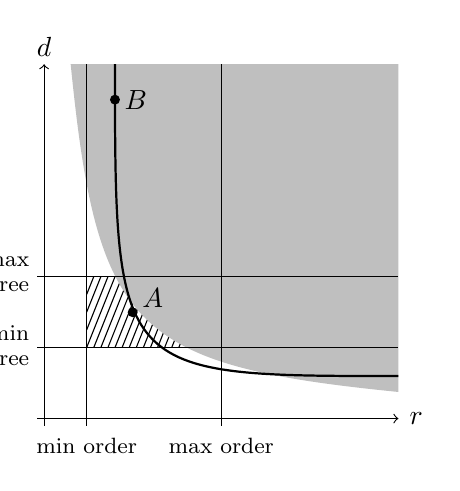
\begin{tikzpicture}[scale=.45]
  \draw[->] (10.5,0) node {$r$} (-.2,0) -- (10, 0) ;
  \draw[->] (0,10.5) node {$d$} (0,-.2) -- (0, 10) ;
  \draw (1.2, 3.5) -- (1.4, 4) (1.2, 3) -- (1.6, 4) (1.2, 2.5) -- (1.8, 4) (1.2, 2) -- (2, 4)
        (1.4, 2) -- (2.2, 4) (1.6, 2) -- (2.4, 4) (1.8, 2) -- (2.6, 4) (2, 2) -- (2.8, 4) 
        (2.2, 2) -- (3, 4) (2.4, 2) -- (3.2, 4) (2.6, 2) -- (3.4, 4) (2.8,2)--(3.6,4) (3,2)--(3.8,4)
        (3.2, 2) -- (4, 4) (3.4, 2) -- (4.2, 4) (3.6, 2) -- (4.4, 4) (3.8,2)--(4.6,4) (4,2)--(4.8,4)
        (4.2, 2) -- (5, 4) (4.4, 2) -- (5.2, 4) (4.6, 2) -- (5.4, 4) (4.8,2)--(5.6,4) (5,2)--(5.8,4); 
  \fill[lightgray] (.75, 10) .. controls (1.5,2.5) and (2.5,1.5) .. (10, .75) -- (10, 10) -- (.75, 10);
  \draw[thick] (2, 10) .. controls (2, 1.2) and (2, 1.2) .. (10, 1.2); 
  \draw (-.2, 2) node {\vbox{\llap{\footnotesize min }\kern-3pt\llap{\footnotesize degree }}} -- (10, 2) 
        (-.2, 4) node {\vbox{\llap{\footnotesize max }\kern-3pt\llap{\footnotesize degree }}} -- (10, 4);
  \draw (1.2, -.2) node {\hbox to0pt{\rule{0pt}{2em}\hss\footnotesize min order\hss}} -- (1.2, 10)
        (5, -.2) node {\hbox to0pt{\rule{0pt}{2em}\hss\footnotesize max order\hss}} -- (5, 10);
  \fill (2.5, 3) circle(4pt) node[right] {\rule[-1em]{0pt}{0pt}$A$} (2, 9) circle(4pt) node[right] {$B$} ;
\end{tikzpicture}}}%
The figure on the right illustrates the typical situation for guessing problems
that are not too small and not too artificial. The light gray region indicates
the area which is not accessible with the given amount of data. Only the points
$(r,d)$ below it can be tested for an operator of order~$r$ and degree~$d$ that
fits to the given data. Let's assume that operators exist on and above the solid
black hyperbola. The user will usually not know this curve in advance but may
have some expectations about it and can restrict the search accordingly, for
example to the dashed area shown in the figure. The method will detect the
existence of an operator, say at point~$A$, and construct from the information
gained at this point an operator of minimal possible order, which may correspond
to point~$B$.  This operator is returned as output. Note that the degree of the
output may exceed the value of \verb|max_degree|, and its order may be smaller
than $\verb|min_order|$:

\begin{sageexample}
sage: data = [(n+1)^10*2^n + 3^n for n in xrange(200)]
sage: L = guess(data, OreAlgebra(ZZ['n'],'Sn'), min_order=3, max_degree=5)
sage: L.order(), L.degree()
\end{sageexample}

In order to test a specific point $(r,d)$, the data array must contain at least $(r+1)(d+2)$ terms. 
If it has more terms, the guess becomes more trustworthy, but also the computation time increases.
By setting the option \verb|ensure| to a positive integer~$e$, the user can request that only 
such points $(r,d)$ should be tested for which the data array contains at least $e$ more terms than
needed. This increases the reliability. By setting the option \verb|cut| to a positive integer~$c$,
the user requests that for testing a point $(r,d)$, the method should take into account at most $c$
more terms than needed. If the data array contains more terms, superfluous ones are ignored in the
interested of better performance. We must always have $0\leq e\leq c\leq \infty$. The default setting
is $e=0$, $c=\infty$. 

Finally, there is an option \verb|infolevel| which, when set to a positive integer, causes the method
to print some output about the progress of the computation. Higher values lead to more detailed output.

\section{Concluding Remarks}

...

 \bibliographystyle{plain}
 \bibliography{main}
 
\end{document}
